\chapter{مقدمه}\label{Chap:Chap1}
\minitoc
همواره زبان به عنوان یکی از پیچیده‌ترین توانایی‌های بشر مورد توجه بوده است. امروزه نیز همچنان توجه بسیاری از محققان به این مسئله است به طوری که حوزه مستقلی در هوش مصنوعی، به نام پردازش زبان طبیعی را به خود اختصاص داده است. پردازش زبان طبیعی شامل
\trans{\task{}}{Task}های
مختلفی مانند،
\trans{تحلیل تمایل}{Semantic Analysis},
\trans{شناسایی موجودیت‌های اسمی}{Named Entity Recognition},
\trans{ترجمه}{Translation},
\trans{پرسش و پاسخ}{Question Answering}
و بسیاری موارد دیگر است. در این بین \task{}
\trans{مدل زبانی}{Language Modeling}
از اهمیت خاصی برخوردار است. اول آنکه با مدل مولد مواجه بوده و علاوه بر این بسیاری از پیچیدگی‌های \task{}‌های دیگر نیز در آن دخیل می‌شود.
مدل‌های زبانی ارائه شده را می‌توان به دو دسته کلی تقسیم نمود. مدل‌های 
\trans{نمادین}{Symbolic}
و مدل‌های آماری. مدل‌های نمادین قدیمی‌تر بوده و بیشتر بر اساس قوانین از پیش تعریف شده کار می‌کنند. این قوانین دقت بالایی در رعایت قوانین دستور زبان دارند اما
\trans{فراخوانی}{Recall}
پایینی دارند؛ چرا که این قوانین تمامی پیچیدگی‌های زبان را مدل نمی‌کنند.\\
در مقابل مدل‌های آماری قرار دارند که پایه آن‌ها مبنی بر پیش‌بینی کلمه بعدی با داشتن کلمه‌های پیشین است که این سبک مدل‌سازی مسئله به مدل‌های 
\trans{خودبرگشتی}{Auto-regressive}
معروف هستند. \\
در دهه اخیر با ظهور
\trans{\gpu{}}{Graphics Processing Unit (GPU)}
و افزایش قدرت محاسباتی ماشین‌ها، آموزش و یادگیری پارامترهای توابع غیرخطی با تعداد لایه‌های زیاد امکان پذیر شده و حوزه‌ای به نام یادگیری ژرف به وجود آمده است؛ برای مثال اخیرا مدل‌هایی با صد میلیون، سیصد میلیون و حتی یک و نیم میلیارد پارامتر آموزش داده و منتشر شده‌اند \cite{bert}. در واقع در هر جایی که به دنبال یادگیری تابعی پیچیده هستیم، می‌توان از یادگیری ژرف بهره برد. به دلیل کاربرد بیشتر و ذات پیوسته تصاویر، بیشتر مدل‌های معرفی شده بر روی تصاویر مورد آزمایش قرار می‌گرفتند. در مقابل به دلیل ذات گسسته متون، حوزه پردازش متن کمی دیرتر در این زمینه رونق گرفت. اما اکنون مدل‌هایی مخصوص پردازش داده‌های دارای حالت دنباله همچون \lstm{} و \transformer{} معرفی شده‌اند که ضمن مدیریت تعداد پارامتر‌ها جملات را به عنوان ورودی دریافت کرده و خروجی متناظر \task{}های مختلف را تولید می‌کنند \cite{transformer, lstm}. در واقع می‌توان هر کلمه را یک متغیر تصادفی در نظر گرفت که مقدار آن نمایانگر کلمه جاری و معمولا تابعی از کلمات پیشین است. روش‌های مورد استفاده برای تولید متن و مدل زبانی، تنها محدود به کاربرد در این حوزه نبوده و در حوزه‌های دیگری همچون تولید گراف، موسیقی، مولکول و هر وظیفه دیگری که حالت دنباله دارد، دارای کاربرد است.\\
اگر بخواهیم مقداری \task{} مدل زبانی را پیشرفته‌تر کنیم، می‌توان این انتظار را داشت که خروجی مدل را کنترل کرد. برای مثال جمله‌ای تولید شود که از کلمات مشخصی تشکیل شده باشد؛ نظری مثبت راجع به یک کالای خاص تولید شود که به این \task{}‌ها، تولید شرطی متن گفته می‌شود. تولید شرطی متن می‌تواند حالات بسیاری را شامل شود؛ از تضمین یک ویژگی در جمله؛ برای مثال مثبت بودن نظر تولید شده تا ترجمه یک جمله از یک زبان به زبان دیگر، همگی شامل مدل‌های مولدی هستند که مشروط به یک مقدار هستند. در مورد اول مشروط به حالت مقصود و درمورد ترجمه نیز مشروط به جمله زبان اولیه است. حتی مدل‌های  مولد بر پایه فضای نهان را نیز می‌توان به عنوان مدل‌های شرطی در نظر گرفت. چرا که جملات تولید شده تابعی از فضای نهان هستند. در اینجا برای مشخص کردن محدوده پروژه،
{\bf
مقصود از تولید شرطی، تولید جملات به شرط مقادیر گسسته و محدود است؛ برای مثال تولید یک جمله در مورد سیاست/ورزش.}
\section{اهمیت و کاربرد}
تولید متن به صورت غیر شرطی هدفی اولیه بوده و برای کاربرد در دنیای واقعی، فاصله داشته و هر گونه امکان کنترل بر روی خروجی مدل به کاربردی‌تر شدن آن کمک خواهد کرد. یک راه حل اولیه می‌تواند آن باشد که به ازای هر شرط یک مدل آموزش داده شود؛ اما چنین معماری به لحاظ تعداد پارامتر مقرون به صرفه نبوده و با افزایش تعداد شرط با مشکل مواجه خواهد شد. بنابراین ارائه مدلی که ضمن رعایت شروط، رعایت محتوا، قالب جمله و همچنین کنترل تعداد پارامتر از اهمیت ویژه‌ای برخوردار است. اگر بخواهیم عملی‌تر صحبت کنیم،تولید متن با محتوای مشخص، 
\trans{\augmentation{}}{Augmentation}
برای مجموعه داده کوچک برچسب‌زده شده، 
\trans{ربات گفت‌گو}{Chatbot}
با قابلیت کنترل موضوع مورد بحث و یا حتی تولید توئیت‌ها و یا اخبار جعلی با جهت‌گیری خاص و غیره را به عنوان کاربرد تولید متن شرطی در نظر گرفت.
\\
به دلیل شباهت ذات این \task{} به بعضی \task{}‌های دیگر، کاربرد تولید متن شرطی محدود به حوزه متن نیست. برای مثال هزینه تولید دارو‌های جدید در ایالت متحده آمریکا عددی فراتر از یک میلیارد دلار است؛ علاوه بر این مدت زمان کشف یک داروی جدید تا عرضه به بازار در حدود ۱۳ سال به طول می‌انجامد. با اینکه کلیه دارو‌های تولید شده تا به حال حدود $10^8$ است اما تعداد کل دارو‌های ممکن عددی در حدود $10^{23}$ تا $10^{60}$ است بنابراین یکی از مراحل ابتدایی و مهم تولید ساختارهای مولکولی اولیه جهت بررسی‌های ماهیت آن‌هاست. با استفاده از روش‌های تولید متن (دنباله) می‌توان با صرف هزینه‌های کمتر، مولکول‌های مختلفی را تولید و رفتار آن‌ها را به عنوان کاندیدا بررسی نمود. واضح است که هرقدر مولکول‌های تولیدی ویژگی‌های مطلوب را بیشتر ارضا کند این هزینه بیشتر کاهش می‌یابد \cite{molecule}. در زمینه تولید موسیفی‌های با هارمونی نیز تلاش‌هایی صورت گرفته است. در این بین استفاده از ساختارهای پیچیده و امکان تولید موسیقی‌های طولانی  و همچنین کنترل سَبک آن نیز مورد توجه است \cite{vae_music, music}.

\section{تعریف مساله} \label{chap1:prob_define}
همان طور که پیش‌تر توضیح داده شد، هر کلمه یک متغیر تصادفی است که هر مقدار آن متناظر با یک کلمه است. یک مدل زبانی غیر شرطی \autoregressive{} را می‌توان به صورت زیر مدل کرد:\\
اگر $X_t$ متغیر تصادفی متناظر با کلمه $t$ام و طول جمله $T$ باشد، طبق قانون زنجیره‌ای خواهیم داشت:
\begin{equation}\begin{split}
		P_\theta(X_1, X_2, ... , X_T) = P_\theta(X_1) P_\theta(X_2|X_1) P_\theta(X_3|X_2, X_1) ... P_\theta(X_T|X_1, ..., X_{T-1})
	\end{split}\end{equation}
که در واقع به دنبال مدل کردن $P_\theta(X_t|X_1, ..., X_{t-1 })$ و یافتن پارامتر‌های $\theta$ هستیم. نمونه برداری از این مدل‌ها نیز به این صورت است که ابتدا کلمه اول از توزیع $P_\theta(X_1)$ نمونه‌برداری شده و سپس کلمه دوم از توزیع $P_\theta(X_2|X_1)$ و سایر کلمات به ترتیب نمونه‌برداری می‌شوند؛ واضح است که به دلیل سبک مدل‌سازی، کلمات بایستی به صورت ترتیبی تولید شوند. \\
نسخه دیگری از تولید دنباله نیز تحت عنوان غیر \autoregressive{} وجود دارد که در مدل‌های زبانی چندان اقبالی نداشته است. این مدل‌ها به این صورت هستند که هر کلمه تابعی از کلمات پیشین خود نیست و تمام کلمات به صورت موازی تولید می‌شوند. برای مثال در کاربرد ترجمه می‌توان فرمول‌بندی زیر را در نظر گرفت:
\begin{align}
	P_\theta(X_1, X_2, ... , X_T|Y) = P_\theta(X_1) P_\theta(X_2|Y) P_\theta(X_3|Y) ... P_\theta(X_T|Y).
\end{align}
که $Y$ جمله زبان مبدا است و کلمات مستقل از یکدیگر و تنها تابعی از جمله مبدأ هستند. مزیت این مدل‌ها در داشتن فاز تولید نمونه سریع‌تر است چرا که کلمه‌ها بر خلاف مدل‌های \autoregressive{} از یکدیگر مستقل هستند و با داشتن $Y$ می‌توان همه را به صورت موازی نمونه‌برداری نمود؛ با این وجود به لحاظ کارایی از مدل‌های \autoregressive{} ضعیف‌ترند. در این پروژه نیز از این دسته از مدل‌ها صرف نظر شده است.
\\
اگر مدل زبانی دارای فضای نهان باشد که با $Z \in \bb{R}^d$ نشان دهیم، مدل زبانی \autoregressive{} دارای فضای نهان را می‌توان به صورت زیر تعریف کرد:
\begin{align}
	P_\theta(X_1, X_2, ... , X_T,Z) = & P(Z) P_\theta(X_1|Z) P_\theta(X_2|X_1,Z) P_\theta(X_3|X_2, X_1,Z) ... \nonumber \\& P_\theta(X_T|X_1, ..., X_{T-1},Z)
\end{align}
و $P(Z)$ به توزیع
\trans{پیشین}{Prior}
شناخته شده و معمولا ثابت است؛ این در حالیست که در بعضی از مدل‌ها این توزیع نیز یاد گرفته می‌شود. برای نمونه‌برداری از این مدل‌ها نیز ابتدا از \priordist{} نمونه‌برداری شده اما بعد، برای نمونه‌برداری کلمات می‌توان پارامتری به نام دما استفاده نمود که مقداری بین صفر و یک دارد و میزان تیز بودن توزیع را کنترل می‌کند و در حالت نزدیک به صفر توزیع را به توزیع $\argmax$ تبدیل می‌کند. این تابع که به \lr{Soft-argmax} معروف است در فصل‌های بعد توضیح داده خواهد شد. بنابراین با داشتن $Z$ می‌توان با پارامتر دما‌های متفاوت از مدل نمونه‌برداری کرد \cite{toward}. شاید معقول باشد که به دنبال
$\argmax_{\bff{x_1}, \bff{x_2}, ..., \bff{x_T}} P_\theta(X_1, X_2, ... , X_T|Z)$
باشیم؛ اما یافتن دنباله با احتمال بیشینه در زمان چندجمله‌ای امکان پذیر نبوده و از \greedydecoding{} که همان استفاده از $\argmax$ در هر زمان است، استفاده می‌شود. در بهترین حالت می‌توان از
\trans{\beamsearch{}}{Beam Search}
بهره برد که به دلیل کُند بودن چندان در مدل‌های زبانی مورد استفاده قرار نگرفته است .
\\
برای تغییر تعاریف فوق به حالت شرطی تنها بایستی توزیع‌ها مشروط گردند. اگر شرط با $C \in \{0,1,2,...K\}$ نشان داده شود، مدل زبانی شرطی بدون فضای نهان به صورت
\begin{align}
	P_\theta(X_1, X_2, ... , X_T|C) = P_\theta(X_1|C) P_\theta(X_2|X_1,C) P_\theta(X_3|X_2, X_1,C) ... P_\theta(X_T|X_1, ..., X_{T-1},C)
\end{align}
و با فضای نهان به صورت
\begin{align}
	P_\theta(X_1, X_2, ... , X_T,Z|C) = & P(Z|C) P_\theta(X_1|Z,C) P_\theta(X_2|X_1,Z,C) P_\theta(X_3|X_2, X_1,Z,C) ... \nonumber \\& P_\theta(X_T|X_1, ..., X_{T-1},Z,C)
\end{align}
تعریف می‌شود.
\section{مدل زبانی با فضای نهان یا بدون فضای نهان؟} \label{chap1:latent_or_not}
مدل‌های زبانی با فضای نهان به این صورت هستند که فرض شده است جملات در فضای نهان ‎کد شده و شبکه 
\trans{‎\decoder{}}{Decoder}یی 
با دریافت برداری از فضای نهان، آن را به جمله مربوطه برگردان می‌کند. با داشتن چنین قابلیتی امکان کنترل کردن شبکه ‎\decoder{}‎ وجود داشته و حتی می‌توان با حرکت روی این فضا جملات شبیه به یکدیگر تولید نموده و یا از یک جمله شروع کرده و به مرور با تغییر بردار ورودی (از فضای نهان) آن به جمله دیگری تبدیل کنیم. این در حالیست که مدل‌های زبانی بدون فضای نهان از این قابلیت بی‌بهره بوده و نمی‌توان کنترلی بر نحوه خروجی آن‌ها داشت \cite{vae_text}.
\section{رویکردهای آموزشی}
به طور کلی دو رویکرد برای آموزش مدل‌های زبانی ارائه شده است. مبتنی بر \likelihood{} و
\trans{\gan{}}{Generative Adversarial Networks}.
در ادامه این دو رویکرد به طور کلی توضیح داده خواهند شد.
\\
{\bf رویکرد مبتنی بر \likelihood{}}:
این رویکرد که به
\trans{\maxlikelihood{}}{Maximum Likelihood}
معروف است، نیاز به محاسبه احتمال جملات در مدل دارد. در حالت مدل بدون فضای نهان، از آنجا که توزیع توام کلمات یک جمله با استفاده از قانون زنجیره‌ای و با کمک احتمال شرطی هر کلمه به کلمات قبل خود بدست می‌آید، بنابراین برای به دست آوردن احتمال یک جمله تنها کافیست احتمال هر کلمه به شرط کلمات قبل خود وجود داشته باشد. لازم به ذکر است که به دلیل محدود بودن واژگان این احتمال به راحتی قابل محاسبه است. بنابراین برای بیشینه کردن \likelihood{} یک جمله در مدل تنها کافیست ضمن ورودی دادن جمله به مدل، در هر زمان احتمال کلمه بعدی بیشینه گردد. این روش آموزش مدل زبانی روش
\trans{\teacherforcing{}}{Teacher Forcing}
نامیده می‌شود \cite{teacher_force}.
\\
در صورتی که مدل دارای فضای نهان باشد، به منظور محاسبه احتمال یک نمونه، نیاز به انتگرال زیر است که به صورت فرم بسته امکان محاسبه آن وجود ندارد و عملا بهینه‌سازی آن به صورت مستقیم امکان‌پذیر نیست.
\begin{align}
	P_\theta(X_1, X_2, ... , X_T) = \int_z P(\bff{z})P_\theta(X_1, X_2, ... , X_T|\bff{z})
\end{align}
از این رو، به جای بیشینه کردن مستقیم \likelihood{}، از مدلی به عنوان تخمینی از توزیع
\trans{\posterior{}}{Posterior}
کمک گرفته و کران پایینی از \likelihood{} که به \lr{ELBO} شناخته می‌شود بیشینه می‌گردد \cite{vae}. این دسته از مدل‌ها
\trans{\vae{}}{Variational Autoencoder}
نامیده می‌شوند. تفاوت این دسته از مدل‌ها به لحاظ ساختاری با
\trans{\autoencoder{}}{Autoencoder}ها
در داشتن توزیع مشخص در فضای نهان و سعی در کم کردن فاصله این توزیع با یک توزیع ثابت، بوده و تفاوت دیگری ندارند.
\\
{\bf رویکرد مبتنی بر \gan{}}:
این رویکرد که جدید‌تر از رویکرد پیشین است، از دو شبکه \generator{} و
\trans{\discriminator{}}{Discriminator}
و یک \minmaxgame{} تشکیل شده است. روند کلی بسیار ساده است. \generator{} سعی در تولید نمونه‌های واقعی داشته و در مقابل \discriminator{} سعی در تشخیص نمونه‌های واقعی از نمونه‌های تولید شده توسط \generator{} دارد \cite{gan}.
\\
\begin{figure}[h]
	\centering
	\begin{subfigure}[b]{1.\textwidth}
		\centering
		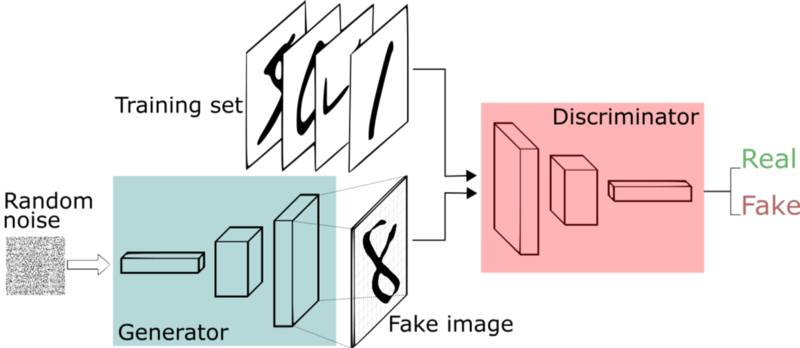
\includegraphics[width=0.7\textwidth]{images/gan.png}
		\caption{}
		\label{fig:gan_arch}
	\end{subfigure}
	\begin{subfigure}[b]{1.\textwidth}
		\centering
		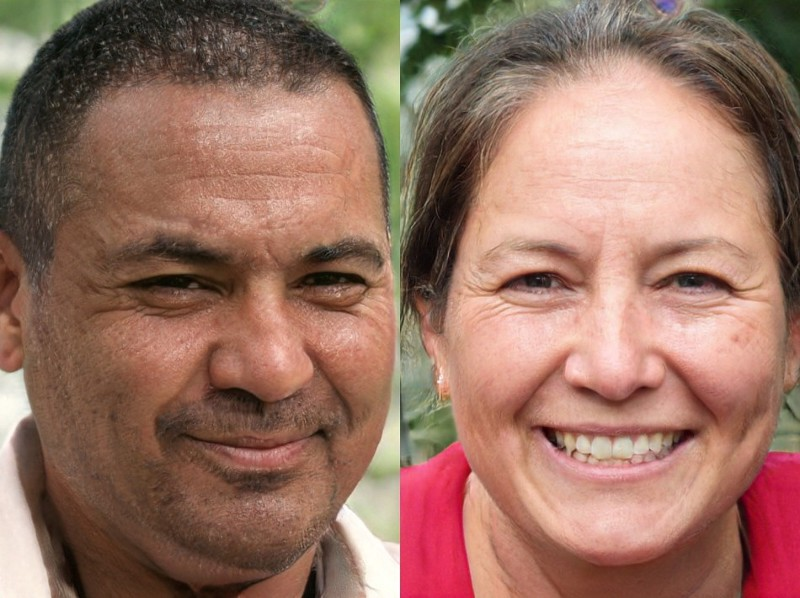
\includegraphics[width=0.5\textwidth]{images/Nvidia/SelectedGenerated.png}
		\caption{}
		\label{fig:gan_sample}
	\end{subfigure}
	\caption{
		روند کلی \gan{}
		(\subref{fig:gan_arch})
		و نمونه تصاویر تولید شده توسط این روش (\subref{fig:gan_sample})
		\cite{gan_nvidia}
	}
\end{figure}
شمایی از نحوه عملکرد این روش در شکل \ref{fig:gan_arch} آمده است؛ همچنین تصاویر شکل \ref{fig:gan_sample} توسط چنین شبکه‌ای تولید شده است که تصاویر بسیار طبیعی هستند.
\\
همان طور که در شکل \ref{fig:gan_arch} مشخص است، شبکه مولد،
\trans{\noise{}}{Noise}
را به تصویر تولید می‌کند. در واقع عامل تصادفی در تصادفی بودن \noise{} اولیه نهفته است. اما در حوزه متن معمولا مدل‌های مولد \noise{}‌ای را دریافت نمی‌کنند چرا که عامل اصلی در نمونه‌گیری هر کلمه در هر زمان وجود داشته و چندان نیازی به \noise{} ورودی نیست.
\section{چالش‌ها} \label{chap1:challenge}
\subsection{ 
    رفتار \meanseeking{} روش \maxlikelihood{}}
از آنجا که در روش \maxlikelihood{} در واقع فاصله $KL(\prob_\text{Data} ~ || Q)$ را کمینه می‌کنیم (زمانی که به دنبال یادگیری $Q$ هستیم)، لازم است تا رفتار مدل در حالتی که ظرفیتی کمتر از پیچیدگی داده دارد را بررسی کنیم. رفتار این فاصله، به گونه‌ای است که Q را به سمتی سوق می‌دهد تا به تمام نقاطی که در $\prob_\text{Data}$ احتمالی دارند، احتمالی نسبت دهد؛ اما نکته نامطلوب آن است که در صورت کمتر بودن ظرفیت مدل نسبت به پیچیدگی داده، برای احتمال نسبت دادن به تمام نقاط داده آموزشی، به نقاطی که در توزیع اصلی داده، احتمالی ندارند نیز احتمال نسبت می‌دهد.
\begin{figure}[h]
	\centering
	\begin{subfigure}[t!]{.4\textwidth}
		\centering
		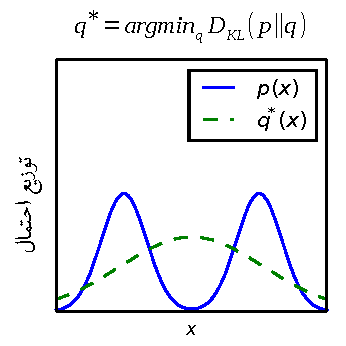
\includegraphics[height=1.\textwidth]{images/KLvsReverseKL_KL.pdf}
		\caption{}
		\label{fig:meanseeking_KL}
	\end{subfigure}
	\begin{subfigure}[t!]{.4\textwidth}
		\centering
		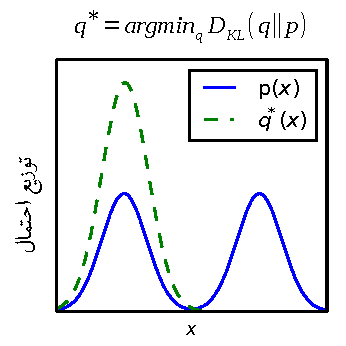
\includegraphics[height=1.\textwidth]{images/KLvsReverseKL_RKL.pdf}
		\caption{}
		\label{fig:meanseeking_RKL}
	\end{subfigure}
	\caption{
		تفاوت رفتار فاصله \lr{KL} (\subref{fig:meanseeking_KL}) و \lr{KL} برعکس (\subref{fig:meanseeking_RKL}) در نحوه یادگیری مدل.
	}
\end{figure}
همان طور که در شکل \ref{fig:meanseeking_KL} دیده می‌شود، ممکن است نقطه‌ای بیشینه احتمال داشته باشد که در توزیع اصلی احتمالی ندارد. به این رفتار روش \maxlikelihood{}، رفتار 
\trans{\meanseeking{}}{Mean Seeking}
 گفته می‌شود. این درحالیست که \lr{KL} برعکس، رفتاری معکوس داشته و در این حالت تنها یکی از قله‌ها را پوشش خواهد داد.
\subsection{ناپایداری و مشکلات \gan{}}
دو مشکل در نحوه آموزش \gan{} نهفته است. اول آنکه با توجه به نحوه آموزش مولد، تنها کافیست مولد نمونه‌ای تولید نماید که \discriminator{} توانایی تشخیص آن از نمونه واقعی را ندهد. در واقع طبیعی بودن نمونه‌ها در روش دیده شده است اما تنوع خیر؛ از سوی دیگر می‌تواند این رفتار به صورت تناوبی بین بعضی نمونه‌ها در حین آموزش جابه‌جا شود. برای مثال اگر هدف یادگیری تصویر قرمز رنگ شکل \ref{fig:gan_train} باشد، ممکن است مسیر آموزش به حالت شکل \ref{fig:gan_bad_train} درآمده و بین بعضی قله‌های داده جابه‌جا شود و از سوی دیگر نیز ممکن است به صورت شکل \ref{fig:gan_good_train} آموزش داده شود که حالتی پایدار است. اگر روند آموزش دچار چنین مشکلی شود، مدل دچار
\trans{\modecollapse{}}{Mode Collapse}
شده است \cite{wgan, gan}.
\begin{figure}[h]
	\centering
	\begin{subfigure}[h]{.7\textwidth}
		\centering
		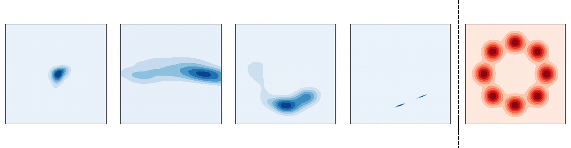
\includegraphics[width=1.\textwidth]{images/GANBadTrain.pdf}
		\caption{}
		\label{fig:gan_bad_train}
	\end{subfigure}
	\begin{subfigure}[h]{.7\textwidth}
		\centering
		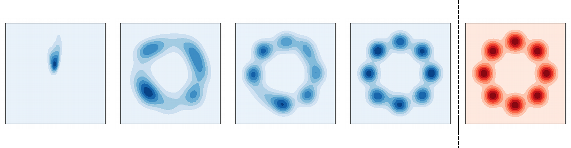
\includegraphics[width=1.\textwidth]{images/GANGoodTrain.pdf}
		\caption{}
		\label{fig:gan_good_train}
	\end{subfigure}
	\caption{
		نمونه‌ای آموزش ناپایدار (\subref{fig:gan_bad_train}) و پایدار
		(\subref{fig:gan_good_train}) \gan{} \cite{numerics_gan}5.
	}
	\label{fig:gan_train}
\end{figure}
\\
مشکل دوم نیز کنترل میزان آموزش \discriminator{} و \generator{} در مقابل یکدیگر است. در صورتی که \discriminator{} بیش از حد آموزش داده شود به طوری که به راحتی نمونه‌های واقعی را از مصنوعی تشخیص دهد، گرادیانی از \discriminator{} به مولد منتقل نشده و آموزش شبکه متوقف خواهد شد. به منظور رفع این مشکل‌ها، راه حل‌های متفاوتی همچون \wgan{}
\LTRfootnote{\lr{Wasserstein Generative Adversarial Network (WGAN)}}
  ارائه شده است \cite{wgan}.
\subsection{عدم توجه به فضای نهان} \label{chap1:latent_ignore}
زمانی که از مدل‌های با فضای نهان استفاده می‌شود، به دنبال یافتن فضای نهانی تفسیرپذیر و تاثیرگذار بر روی خروجی \decoder{} هستیم؛ اما در صورت بالا بودن ظرفیت \decoder{} ممکن است مستقل از فضای نهان، توزیع داده اصلی را فرا بگیرد. در این صورت فضای نهان نه تفسیرپذیر و نه تاثیرگذار بر روی خروجی \decoder{} بوده و عملا با یک مدل زبانی بدون فضای نهان برابری خواهد کرد. این مشکل نیز مورد توجه محققان بوده و روش‌های متفاوتی از جمله \wae{}
 \LTRfootnote{\lr{Wasserstein Autoencoder (WAE)}}
  ارائه شده است \cite{wae, infovae, vae_lagging, vae_lossy}.
\subsection{گذر گرادیان در نمونه‌برداری و \argmaxphrase{}}
از آنجا که در حوزه مدل زبانی با نمونه‌گیری از توزیع کلمات سر و کار داریم، در روش‌هایی مانند \gan{} با مشکل مواجه خواهیم بود. در واقع به دلیل اینکه نمونه‌گیری عملیاتی مشتق نا‌پذیر است، امکان گذر گرادیان از این عملیات به عقب وجود ندارد. برای مثال در روش \gan{}، تابع هدف مدل مولد، تولید نمونه‌هاییست که از نظر \discriminator{} واقعی به نظر رسند. بنابراین بایستی از مولد نمونه‌برداری کرده و سپس احتمال واقعی بودن نمونه‌ها توسط \discriminator{} ارزیابی شود. حال برای آموزش دادن پارامتر‌های مولد نیاز است تا گرادیان از \discriminator{} به مولد منتقل گردد؛ اما در این مسیر عملیات نمونه‌برداری وجود دارد. مشکل مشابهی نیز هنگام 
\trans{\argmaxphrase{}}{Argmax}
 رخ می‌دهد. برای رفع این مشکل نیز راه‌حل‌هایی همچون بهره‌گیری از یادگیری تقویتی و یا روش‌هایی تقریبی همچون \lr{Gumbel Softmax} و \lr{Soft-argmax} ارائه شده‌اند اما روش یادگیری تقویتی واریانس گرادیان را افزایش داده و روش‌های تقریبی نیز دارای پارامتر‌هایی هستند که تنظیم آن‌ها نیازمند توجه و دقت است \cite{seqgan, gumbel}
\subsection{عدم تطابق شرط با جمله تولیدی}
مشکل دیگری که ممکن است در روش‌های مبتنی بر \likelihood{} پیش آید، احتمال ناهمخوانی شرط با جمله تولیدی است. از آنجا که معمولا تطابق جمله خروجی با شرط چک نمی‌شود، ممکن است این اتفاق نامطلوب رخ دهد. لازم به ذکر است که در روش \gan{} انتظار چنین رخدادی وجود ندارد چرا که این موضوع توسط \discriminator{} تصحیح می‌شود \cite{toward}.
\section{هدف پژوهش}
با توجه به تعریف مسئله در بخش \ref{chap1:prob_define} و چالش‌های معرفی شده در بخش \ref{chap1:challenge} به دنبال ارائه روشی برای آموزش شبکه‌های مولد شرطی بوده که کمتر با چالش‌های ارائه شده مواجه شود و جملات تولیدی چه به لحاظ کیفیت و چه به لحاظ تطابق با شرط از سطح قابل قبولی برخوردار باشند.
\\
به این منظور  سعی در آموزش مدل مولد با فضای نهان شرطی به طوری که فضای نهان به ازای مقادیر مختلف شرط، تقسیم گردد و همچنین استفاده از روش‌هایی همچون \wae{} برای جلوگیری از مشکل عدم توجه به فضای نهان خواهیم داشت. علاوه بر این از معماری‌های نوینی همچون \transformer{} و رویکرد‌های آموزش مدل‌های مولدی که کمتر مورد توجه بوده‌اند اما ویژگی‌های متناسب با فضای مسئله را دارند، استفاده خواهد شد.

\section{ساختار پایان‌نامه}
در فصل \ref{chap2}، پس از معرفی تعدادی فاصله بین توزیع‌های به عنوان پیشنیاز، به دلیل شباهت مدل‌های زبانی شرطی به غیر شرطی، ابتدا مدل‌های غیر شرطی تحت عنوان مدل‌های با فضای نهان و بدون فضای نهان تشریح شده و در انتها نیز معماری نوینی تحت عنوان \transformer{} معرفی می‌گردد. از آنجا که در روش پیشنهادی از نوعی مدل‌های مولد که پیش‌تر مورد توجه نبوده‌اند استفاده گردیده است، به معرفی این دسته از مدل‌های مولد نیز پرداخته خواهد شد. در فصل \ref{chap3} نیز پس از بررسی اجمالی مدل‌های معرفی شده، مدل پیشنهادی ارائه شده و در فصل  \ref{chap4} پس از معرفی داده و معیارهای ارزیابی مورد بررسی قرار گرفته و نتایج گزارش شده است. در نهایت نیز ضمن ارائه جمع‌بندی از کارهای انجام شده، پیشنهاداتی جهت ادامه تحقیقات معرفی خواهد شد.




